\section{Mathematical model of a quadcopter}\label{sec:model}
In this section, the mathematical model of a quadcopter is presented, mainly based on \cite{quad_model}. Firstly, the coordinate frames are characterized to describe the position and orientation of the drone. The dynamic equations are then written in these frames for translational and rotational motion using multiple attitude representations. Finally, the input equations are described which define a mapping between the control inputs and propeller angular velocities.

\subsection{Coordinate frames}\label{sec:frames}
In order to derive the dynamical model or assign the coordinate frames, first the configuration of the quadcopter has to be fixed. The configuration defines the placement and the direction of rotation of the rotors thus basically determines the structure of the dynamical model and the control strategy. The most commonly used configurations are denoted by '+' and '$\times$', which differ only in the assignment of the front of the vehicle (see Figure~\ref{fig:frames}). Due to practical considerations (e.g. camera placement) the earlier is more common, therefore we use '$\times$' configuration in this work.

After the configuration is fixed, the coordinate frames can be clearly defined. Three main frames are introduced: the inertial frame $\mathcal{F}^i$ interpreted as NED (north-east-down) coordinates, the vehicle frame $\mathcal{F}^v$, and the body frame $\mathcal{F}^b$, which is fixed to the vehicle. The three frames are displayed in Figure~\ref{fig:frames}, with the body frame both in '$\times$' and '+' configuration. The transformation from $\mathcal{F}^i$ to $\mathcal{F}^v$ is a translation, and from $\mathcal{F}^v$ to $\mathcal{F}^b$ a rotation. In the figure, the rotation is described by the roll, pitch, and yaw (RPY) Euler angles, denoted by $\phi$, $\theta$, and $\psi$, respectively. However, we will also present other techniques to characterize this rotation in Section \ref{sec:rotation}.

\begin{figure}[b]
\centering 
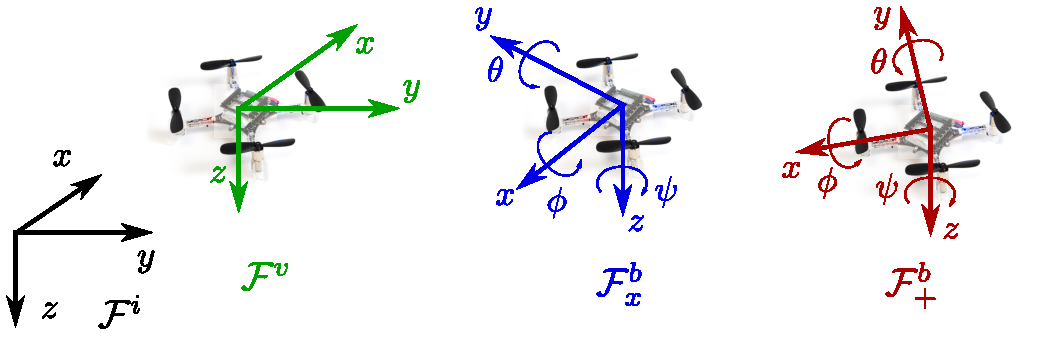
\includegraphics[width=.75\textwidth]{Fig/xconf.pdf}
\caption[Inertial, vehicle, and body frames]{Inertial, vehicle, and body frames describing the geometric relations of the vehicle and the environment. The body frame is depicted both in '$\times$' and '+' configurations.}\label{fig:frames}
\end{figure}

The matrix representation of the transformation between the vehicle and body frames can be derived from the RPY angle representation as follows:
\begin{equation}\label{eq:rot}
\begin{split}
R_v^b& = Rot(x,\phi)Rot(z,\theta)Rot(z,\psi) = \\
&=\left[\begin{array}{ccc}1 & 0 & 0 \\ 0 & C_ \phi &  S_ \phi \\ 0 & - S_ \phi & C_ \phi\end{array}\right]\left[\begin{array}{ccc} C_ \theta & 0 &  -S_ \theta \\ 0 & 1 & 0 \\  S_ \theta & 0 &  C_ \theta\end{array}\right]\left[\begin{array}{ccc} C_ \psi & S_ \psi & 0 \\ - S_ \psi &  C_ \psi & 0 \\ 0 & 0 & 1\end{array}\right]=\\
&=\left[\begin{array}{ccc} C_\psi C_\theta &  C_\theta S_\psi & -S_\theta \\
C_\psi S_\phi S_\theta - C_\phi S_\psi & C_\phi C_\psi + S_\phi S_\theta S_\psi & S_\phi C_\theta \\
S_\phi S_\psi + C_\phi C_\psi S_\theta & C_\phi S_\theta S_\psi - C_\psi S_\phi & C_\phi C_\theta
\end{array}\right],     %\left[\begin{array}{ccc} C_\psi C_\theta &  C_\theta S_\psi+ C_\psi S_\phi S_\theta &  S_\phi S_\psi- C_\phi C_\psi S_\theta \\ -C_\theta S_\psi &  C_ \phi C_ \psi - S_\phi S_\psi S_\theta & C_\psi S_\phi + C_\phi S_\psi S_\theta \\ S_\theta &  -C_\theta S_ \phi &  C_ \phi C_\theta\end{array}\right],
\end{split}
\end{equation}
where $C_\cdot = \cos(\cdot)$, $S_\cdot = \sin(\cdot)$, and $R_v^b$ is called the rotation matrix. The coloumn vectors of the rotation matrix formulate an orthonormal basis of the 3D space, therefore
\begin{equation}
R_b^v = \left(R_v^b\right)^{-1} = \left(R_v^b\right)^\top.
\end{equation}

\subsection{Translational dynamics}\label{sec:trans}

The vehicle can be modelled as a rigid body with mass and inertia in the 3D space, on which gravity field acts. The active movement of the drone is generated by  four electric motors and the propellers on them. They produce a collective thrust applied in the center of mass of the vehicle, and three moments around the three coordinate axes.

The translational dynamics of the quadcopter are characterized by Newton's equations of motion, generally expressed as
\begin{equation}\label{eq:newton}
f= m\frac{\mathrm{d} V}{\mathrm{d} t_i},
\end{equation}
where $f$ is the vector of forces acting on the mass $m$, and $V$ is the velocity of the mass. The notation $t_i$ expresses that the derivative is calculated with respect to the inertial frame.

In our model, there are two forces acting on the vehicle: the collective thrust generated by the motors, and the force of the gravitational field. The collective thrust always points in the negative $z$ direction of the body frame, and gravity always points in the positive $z$ direction of the inertial frame. The force vector in \eqref{eq:newton} results from these terms, as
\begin{equation}\label{eq:newtoneq}
f = R_b^v\begin{bmatrix} 0\\0\\-F \end{bmatrix} + \begin{bmatrix} 0\\0\\mg \end{bmatrix},
\end{equation}
where $F$ is the collective thrust of the propellers, and $g$ is the gravitational acceleration.
\newpage
\subsection{Rotational dynamics} \label{sec:rotation}

There are multiple ways to describe the rotational motion of a rigid body in 3D space, three of which are presented in this work. The most common and simple way is to use local coordinates to describe the attitude with three axes, and three rotation angles around them. An example is the RPY angle representation mentioned in Section \ref{sec:frames}, where the three axes are the body $z, y, x$ axes, and the three angles are the yaw ($\psi$), pitch ($\theta$) and roll ($\phi$), respectively. Although this approach is intuitive and commonly used, it has two major drawbacks. The first is that it is only valid in a certain region of the attitude, for example $-\pi/2 \leq \phi \leq \pi/2,\; -\pi/2 \leq \theta \leq \pi/2,\; 0 \leq \psi \leq 2\pi$. The second is the so called \textit{gimbal lock}, meaning that a degree of freedom is lost if two axes become parallel out of the three. In case of the flip maneuver, when the pitch is 90 degrees, the yaw axis is parallel to the roll axis, and the compensation for the yaw changes is not possible. Due to these drawbacks, RPY (or Euler) angles are used only for slower maneuvering and trajectory tracking, but for aggressive maneuvers other,  more suitable modelling approaches are needed.

Another possible representation of rigid body rotations is using quaternions. In this case, there is no need to deal with the gimbal lock, and a continuous trajectory can be described by a continuous function of the quaternion elements. However, unit quaternions are ambiguous, as they double-cover the rotation group $SO(3)$, meaning that quaternions $q$ and $-q$ represent the same rotation which causes difficulties in control design. Therefore we use this representation only for reference trajectory design.

The third representation of orientation we describe is the rotation matrix. Any rigid body rotation can be characterized by a $3\times 3$ orthogonal matrix with determinant 1. These matrices form the configuration space of the orientation of a non-symmetrical object in 3D space, named the special orthogonal group, $SO(3)$. Advantages of this approach are that the product of two rotations is the composition of the rotations, therefore the orientation can be given as the rotation from an initial frame to a current body frame, and it avoids singularities and complexities arising when using local coordinates. The disadvantages of using orientation matrices are that the use of 9 variables (elements of a $3\times 3$ matrix) is computationally less efficient than 3 angles or 4 quaternion elements, and they are less illustrative.

In this section, the rotational dynamics of the quadrotor is derived using all three mentioned representations, in order to be able to use them for trajectory planning and control design. The translational dynamics from Section \ref{sec:trans} and the rotational dynamics with one of the three attitude representations together characterize the dynamic model of the quadcopter.

\subsubsection{Euler angles}
The orientation is described with the vector of roll, pitch and yaw angles, $[\phi,\theta,\psi]^\top$. However, since the three rotations are in different frames, the vector of derivatives of the three angles is not equal to the derivative of the vector of the angles. We denote the former $[\dot\phi,\dot\theta,\dot\psi]^\top$, and the latter $[p,q,r]^\top$. The relation of these vectors is described by a matrix transformation, as
\begin{align}
\begin{bmatrix} p\\q\\ r \end{bmatrix} &= \begin{bmatrix}
1 & 0 & -\sin\theta \\ 
0 & \cos\phi & \cos\theta\sin\phi \\ 
0 & -\sin\phi & \cos\theta\cos\phi
\end{bmatrix}\begin{bmatrix}
\dot\phi \\ \dot\theta \\ \dot\psi
\end{bmatrix} = W \begin{bmatrix}
\dot\phi \\ \dot\theta \\ \dot\psi
\end{bmatrix},\\
\begin{bmatrix}
\dot\phi \\ \dot\theta \\ \dot\psi
\end{bmatrix}&= W^{-1}\begin{bmatrix} p\\q\\ r \end{bmatrix} = \begin{bmatrix}
1 & \sin\phi\tan\theta & \cos\phi\tan\theta \\
0 & \cos\phi & -\sin\phi \\
0 & \frac{\sin\phi}{\cos\theta} & \frac{\cos\phi}{\cos\theta}
\end{bmatrix}\begin{bmatrix} p\\q\\ r \end{bmatrix}.\label{eq:angvel}
\end{align}

The rotational dynamics can be described by Euler's equations, as
\begin{equation}\label{eq:newton2}
\tau = \frac{\mathrm{d}J\omega}{\mathrm{d}t_i},
\end{equation}
where $\tau$ is the torque acting on the body, $J$ is the inertia, and $\omega$ is the angular velocity. The rotation is easier to express in the body frame, as the $J^b$ inertia is constant, and the angular velocity is $\omega^b = [p,q,r]^\top$. However, as the derivatives in \eqref{eq:newton2} are calculated with respect to the inertial frame, the formulae of derivation in a moving frame have to be applied, resulting in
\begin{align}
\frac{\mathrm{d}J^b\omega^b}{\mathrm{d}t_i}&= \frac{\mathrm{d}J^b\omega^b}{\mathrm{d}t_b} + \left(\omega^b\times J^b \omega^b\right)=\underbrace{\frac{\mathrm{d}J^b}{\mathrm{d}t_i}\omega^b}_{=0} + J^b \frac{\mathrm{d}\omega^b}{\mathrm{d}t_i} + \left(\omega^b\times J^b \omega^b\right) = \tau,\\
    &\Downarrow \nonumber\\
\begin{bmatrix}
\dot{p} \\ \dot{q} \\ \dot{r} 
\end{bmatrix} &= \left(J^b\right)^{-1}\left(\tau - \omega^b\times J^b \omega^b\right) .\label{eq:rot_dyn}
\end{align}

Quadcopters are almost perfectly symmetric, therefore the off-diagonal terms of the inertia matrix are usually neglected. Thus the equation for the rotational acceleration results in
\begin{equation}\label{eq:rotvel}
\begin{bmatrix}
\dot{p} \\ \dot{q} \\ \dot{r} 
\end{bmatrix} = \begin{bmatrix}
\frac{J_y-J_z}{J_x}\cdot q\cdot r + \frac{\tau_x}{J_x} \\ \frac{J_z-J_z}{J_x}\cdot p\cdot r + \frac{\tau_y}{J_y} \\ \frac{J_x-J_y}{J_z}\cdot p\cdot q  + \frac{\tau_z}{J_z}  
\end{bmatrix}.
\end{equation}

The drone as a rigid body in 3D space has 12 states: the position, velocity, rotation and rotational velocity. The equations for the velocity are from \eqref{eq:rot} and \eqref{eq:newtoneq}, for the rotation from \eqref{eq:angvel}, and for the rotational velocity from \eqref{eq:rotvel}. Gathering these to a matrix form, the following state space representation is formulated:
\begin{equation}\label{eq:ss}
\begin{bmatrix}
\dot{x} \\ \dot{y} \\ \dot{z} \\ \dot{V_x} \\ \dot{V_y} \\ \dot{V_z} \\ \dot{\phi} \\ \dot{\theta} \\ \dot{\psi} \\ \dot{p} \\ \dot{q} \\ \dot{r}
\end{bmatrix} = \begin{bmatrix}
V_x \\ V_y \\ V_z \\ -(\sin \phi \cdot \sin \psi+\cos \phi \cdot \cos \psi \cdot \sin \theta) \frac{F}{m} \\
-(\cos \phi \cdot \sin \psi \cdot \sin \theta-\cos \psi \cdot \sin \phi) \frac{F}{m} \\
-(\cos \phi \cdot \cos \theta) \frac{F}{m}+g \\
p+\sin \phi \cdot \tan \theta \cdot q+\cos \phi \cdot \tan \theta \cdot r \\
\cos \phi \cdot q-\sin \phi \cdot r \\
\frac{\sin \phi}{\cos \theta} \cdot q+\frac{\cos \phi}{\cos \theta} \cdot r \\
\frac{J_{y}-J_{z}}{J_{x}} \cdot q \cdot r+\frac{\tau_{x}}{J_{x}} \\
\frac{J_{z}-J_{x}}{J_{y}} \cdot p \cdot r+\frac{\tau_{y}}{J_{y}} \\
\frac{J_{x}-J_{y}}{J_{z}} \cdot p \cdot q+\frac{\tau_{z}}{J_{z}}
\end{bmatrix}.
\end{equation}


\subsubsection{Quaternion based model}
%The so far described RPY representation is only valid for a certain region of the angles, i.e. $-\pi/2 \leq \phi \leq \pi/2,\; -\pi/2 \leq \theta \leq \pi/2,\; 0 \leq \psi \leq 2\pi$. It is sufficient in most cases, e.g. following a path or slower maneuvering, but in case of an aggressive maneuver, another approach would be more convenient. Using quaternions for describing rotations is a possible solution for the problem \cite{quaternion,energy-quaternion}. 
The second presented approach for rigid body attitude representation is using quaternions. A quaternion is a hyper complex number of rank 4, which can be represented in multiple forms, see for example equation \eqref{eq:q1}. The quaternion elements from $q_1$ to $q_3$ are called the vector part of the quaternion, while $q_0$ is the scalar part.
\begin{align}
    q = q_0 + q_1\mathbf{i} + q_2\mathbf{j} + q_3\mathbf{k} = \begin{bmatrix}q_0 & q_1 &q_2& q_3 \end{bmatrix}^\top = \begin{bmatrix}q_0 \\ \mathbf{q} \end{bmatrix} \label{eq:q1}
\end{align}
Quaternions have a special multiplication operator, denoted by $\otimes$. If $p$ and $q$ represent rotations, $p\otimes q$ represents the combined rotation. Just as the rotation, quaternion product is not commutative. Two possible (equivalent) methods for calculating this product are the following.
\begin{align}
    p\otimes q &= \underbrace{p_0 q_0 - \mathbf{p}\cdot\mathbf{q}}_{\mathrm{scalar\; part}} +\underbrace{p_0 \mathbf{q} +q_0\mathbf{p} + \mathbf{p}\cross\mathbf{q}}_{\mathrm{vector\; part}},\\
    p\otimes q &= Q(p) q=\left[\begin{array}{cccc}
p_{0} & -p_{1} & -p_{2} & -p_{3} \\
p_{1} & p_{0} & -p_{3} & p_{2} \\
p_{2} & p_{3} & p_{0} & -p_{1} \\
p_{3} & -p_{2} & p_{1} & p_{0}
\end{array}\right]\left[\begin{array}{l}
q_{0} \\
q_{1} \\
q_{2} \\
q_{3}
\end{array}\right] = \left[\begin{array}{l}
p_{0} q_{0}-p_{1} q_{1}-p_{2} q_{2}-p_{3} q_{3} \\
p_{0} q_{1}+p_{1} q_{0}+p_{2} q_{3}-p_{3} q_{2} \\
p_{0} q_{2}-p_{1} q_{3}+p_{2} q_{0}+p_{3} q_{1} \\
p_{0} q_{3}+p_{1} q_{2}-p_{2} q_{1}+p_{3} q_{0}
\end{array}\right].
\end{align}

Rotations are defined by unit quaternion products, i.e. the definition of a norm is necessary, as
\begin{align}
    \norm{q} = \sqrt{q_0^2+q_1^2+q_2^2+q_3^2}.
\end{align}
The complex conjugate of a quaternion will also be needed, defined as
\begin{align}
    q^* = \begin{bmatrix}q_0 & -q_1 & -q_2 & -q_3 \end{bmatrix}^\top.
\end{align}
Given that the angular velocity is in the body frame, the derivative of the quaternion rotation in the dynamic equations has the form \cite{quaternion}
\begin{align}
    \dot{q} =-\frac{1}{2} \omega^b \otimes q.
\end{align}
It is worth noting that if we apply the quaternion product to a $\mathbb{R}^3$ vector and a quaternion, the scalar part of the vector is always considered zero.

The rotation in \eqref{eq:newtoneq} can be characterized by two quaternion products, namely
\begin{align}
    f = q\otimes\begin{bmatrix}0 \\ 0 \\ -F\end{bmatrix}\otimes q^* + \begin{bmatrix}0 \\ 0 \\ mg\end{bmatrix},
\end{align}
where $q$ is the rotation quaternion between the inertial and body frame.

The state space representation using \eqref{eq:ss} and the above expressions has the following form:

\begin{equation}\label{eq:quatss}
\def\arraystretch{1.5}
\begin{bmatrix}
\dot{r} \\ \dot{V} \\ \dot{q} \\ \dot{\omega}^b
\end{bmatrix} = \left[\begin{array}{c}
V \\ q\otimes\frac{1}{m}\def\arraystretch{1}\begin{bmatrix}0 \\ 0 \\ -F \end{bmatrix}\otimes q^* + \begin{bmatrix}0 \\ 0 \\ g\end{bmatrix} \\ -\frac{1}{2} \omega^b \otimes q \\\left(J^b\right)^{-1}\left(\tau - \omega^b\times J^b \omega^b\right)
\end{array} \right].
\end{equation}

\subsubsection{Rotational dynamics on $SO(3)$}
Although it is possible to describe any rotation with quaternions, ambiguities arise when using them to represent the attitude. The third orientation representation method described is the quadcopter model on the special orthogonal group, $SO(3)$. The proper mathematical background of group theory and Lie-groups for rigid body orientation can be found for example in \cite{isidori1995nonlinear,Leethesis}. In this paper, only the most important principles are described with an emphasis on applications.

The\textit{ orthogonal group }$O(n)$ is the group of $n\times n$ orthogonal matrices, with the following property: 
\begin{align}
    A\in O(n) \Leftrightarrow AA^\top=I,
\end{align}
where $A$ is an $n\times n$ matrix. The column vectors of these matrices are orthogonal, and their determinant is always either 1 or $-1$. The\textit{ special orthogonal group} $SO(n)$ is the subgroup of orthogonal matrices, in which every matrix has determinant 1. These matrices can represent rotations in $n$-dimensional space, therefore they are named rotation matrices.
%In order to represent both translations and rotations, $SO(n)$ needs to be extended. Consider the set of all $(n+1)\times (n+1)$ transformation matrices of the form
%\begin{align}
%    \left\{ \begin{pmatrix}R & v \\ 0 & 1  \end{pmatrix} \;\bigg\vert\; R \in SO(n) \mbox{ and } v \in {\mathbb{R}}^n \right\}.
%\end{align}
%The matrix $R$ achieves the rotation, and the vector $v$ the translation. The result is the \textit{special Euclidean group} $SE(n)$, which is homeomorphic to $ {\mathbb{R}}^n \times SO(n)$, because the rotation matrix and translation vectors may be chosen independently.
%Rigid body translation and rotation is described in the 3D space, therefore the representation is in the special Euclidean group $SE(3)$, and the rotation matrix in the special orthogonal group $SO(3)$. 
The attitude dynamics have a simple form using rotation matrices, namely
\begin{subequations}\label{eq:rot12}
   \begin{align}
    \dot{R}_v^b & = R_v^b\hat{\omega}^b,\label{eq:rot1}\\
    \dot{\omega} & = \left(J^b\right)^{-1}\left(\tau - \omega^b\times J^b \omega^b\right),\label{eq:rot2}
\end{align} 
\end{subequations}
where $R_v^b\in SO(3)$ is the rotation matrix between the vehicle and body frames, and the \textit{hat map} $\hat{\cdot}:\mathbb{R}^3\rightarrow SO(3)$ is defined by the condition that $\hat{x}y = x\times y$ for all $x,y\in \mathbb{R}^3$. From here on the indices corresponding to the body and vehicle frames from \eqref{eq:newtoneq} and \eqref{eq:rot_dyn} are omitted for clarity, the inertia and angular velocity are always defined in the body frame. %The translational dynamics are characterized by \eqref{eq:newtoneq}, the two forces acting on the body are the collective thrust and gravitational force.
%\subsection{Differential flatness}\label{sec:flat}
%The demonstrated dynamical model of the quadcopter is underactuated as it has six degrees of freedom and only four control inputs. However, in trajectory design it is often utilized that the model is \textit{differentially flat}, i.e. all state variables and control inputs can be expressed from a finite number of time derivatives of four flat outputs, namely the position $x,y,z$ and yaw angle $\psi$. This simplifies the trajectory planning: only $x_d(t), y_d(t), z_d(t), \psi_d(t)$ have to be constructed, they determine the remaining states. 

\subsection{Input equations}
The dynamic model has four inputs: the collective thrust, and the torques around the three axes of the body frame. These inputs can be calculated from the individual thrusts and angular speeds of the actuators, the equations of which are described in this section.

The thrust generated by each motor ($T_i$) is proportional to the square of the corresponding angular velocity ($\omega_i$), resulting in the equation
\begin{equation}
T_i = k\omega_i^2,\label{eq:thrustconstant}
\end{equation}
where $k$ is the \textit{thrust constant}. 

% \subsubsection{'X' configuration}

The direction of rotor thrust, angular velocity and the numbering of propellers are displayed in Figure \ref{fig:input_eqs}. The torques around the axes $x$ and $y$ can be calculated as the product of the thrusts $T_i$, and the distance of the motors and the center of mass of the vehicle $l$, as
\begin{align}
\tau_x &= \frac{l}{\sqrt{2}}(T_3+T_4-T_1-T_2) =  \frac{l}{\sqrt{2}} k \left(\omega_3^2+\omega_4^2-\omega_1^2-\omega_2^2\right),\\
\tau_y &= \frac{l}{\sqrt{2}}(T_1+T_4-T_2-T_3) =  \frac{l}{\sqrt{2}}k \left(\omega_1^2+\omega_4^2-\omega_2^2-\omega_3^2\right).
\end{align}
The torque around axis $z$ is calculated based on the effect, that every propeller rotates the vehicle in the opposite direction, and this rotating torque is proportional to the square of the angular velocity. Therefore rotors 1 and 3 create positive torque, and the others negative, resulting in the equation
\begin{equation}\label{eq:dragconstant}
\tau_z = b\left(\omega_1^2+\omega_3^2-\omega_2^2-\omega_4^2\right),
\end{equation}
where $b$ is the \textit{drag constant}. We can write the input equations \eqref{eq:thrustconstant}--\eqref{eq:dragconstant} in a matrix form, resulting in
\begin{align}\label{eq:inputs}
\begin{bmatrix}F \\ \tau\end{bmatrix}=\begin{bmatrix}1 & 1 & 1 & 1 \\ -\frac{l}{\sqrt{2}} &  -\frac{l}{\sqrt{2}} &  \frac{l}{\sqrt{2}} &  \frac{l}{\sqrt{2}} \\  \frac{l}{\sqrt{2}} & -\frac{l}{\sqrt{2}} &  -\frac{l}{\sqrt{2}} &  \frac{l}{\sqrt{2}} \\ \frac{b}{k} & -\frac{b}{k} & \frac{b}{k} & -\frac{b}{k}\end{bmatrix}\begin{bmatrix} k \omega_{1}^{2} \\ k \omega_{2}^{2} \\ k \omega_{3}^{2} \\ k \omega_{4}^{2}\end{bmatrix}.
\end{align}

\begin{figure}
\centering 
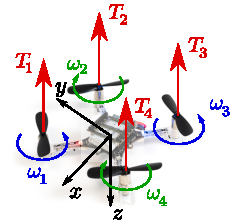
\includegraphics[width=.3\textwidth]{Fig/input_eqs.pdf}
\caption{Thrusts and angular velocities of the rotors with the body frame.}\label{fig:input_eqs}
\end{figure}

% \subsubsection{'+' configuration}
% In this case, the moments around $x$ and $y$ axes depend only on the thrust or angular velocity of two rotors, and the moment around $z$ does not differ from the previous case. The form of the equations are
% \begin{align}
% \tau_x &= l(T_4-T_2) =  l k \left(\omega_4^2-\omega_2^2\right),\\
% \tau_y &= l(T_1-T_3) = l k \left(\omega_1^2-\omega_3^2\right), \\
% \begin{bmatrix}F \\ \tau\end{bmatrix}&=\begin{bmatrix}1 & 1 & 1 & 1 \\ 0 &  -l &  0 &  l \\  l & 0 &  -l &  0 \\ \frac{b}{k} & -\frac{b}{k} & \frac{b}{k} & -\frac{b}{k}\end{bmatrix}\begin{bmatrix} k \omega_{1}^{2} \\ k \omega_{2}^{2} \\ k \omega_{3}^{2} \\ k \omega_{4}^{2}\end{bmatrix}.
% \end{align}

Since there is a constant mapping between the motor angular velocity and the vector of collective thrust and moments, we consider the $\left[F,\; \tau^\top\right]^\top$ vector the input of the system.

The identification of the input parameters $k$ and $b$ are important for accurate simulation-to-reality transfer, however, it is often difficult due to the complex aerodynamic effects, such as blade flapping and downwash. These parameters are usually determined experimentally. It is important to note, that precise modelling of the actuation mechanism often requires more complex dynamical models than \eqref{eq:thrustconstant} and \eqref{eq:dragconstant} \cite{Forster}.  In the methods presented we use only the simplified model, although we point out in Section~\ref{sec:simu} that increasing the accuracy of the model improves the performance of the control algorithms.
%The connection of rotor angular velocity, rotor thrust and torque are often determined experimentally, resulting in more complex models than the equations described by \eqref{eq:thrustconstant} and \eqref{eq:dragconstant} \cite{Forster}.